Concepts and initial ideas of the CloudMan project are described in~\cite{CloudManProject}. The purpose of this document is to define interfaces and the design of the modules, aiming at the implementation of the tool. An overview over the architecture is given in fig.~\ref{architecture}, as described in ~\cite{CloudManProject}.

As a general guideline, standard OpenSource tools and frameworks, and/or existing services should be used where ever possible. 

\begin{figure}
\begin{center}
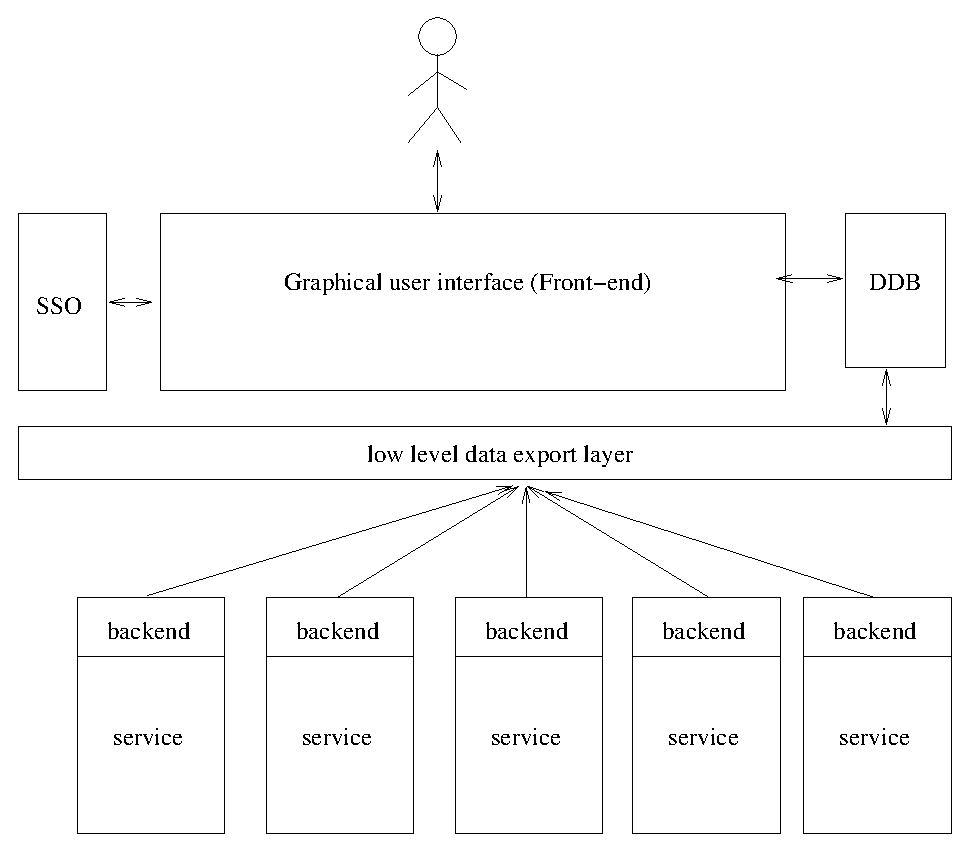
\includegraphics[width=0.9\textwidth]{architecture2.eps}
\caption{\label{architecture} Basic architecture of the desired system. Users connect to the front-end which offers a graphical user interface. They authenticate using the site Single Sign On mechanism or similar. The data which is entered is stored in an external database, and exported in a low level format. Back-ends which are design to configure specific services, for example local cloud installations, consume this information to configure their resources.}
\end{center}
\end{figure}

